%Appendices
\begin{appendices}
	\renewcommand{\thechapter}{\Roman{chapter}}
\chapter{Process Flow diagrams}\label{Schematics}
\newpage
	
	\begin{figure}[h!]
		\centering
		\fbox{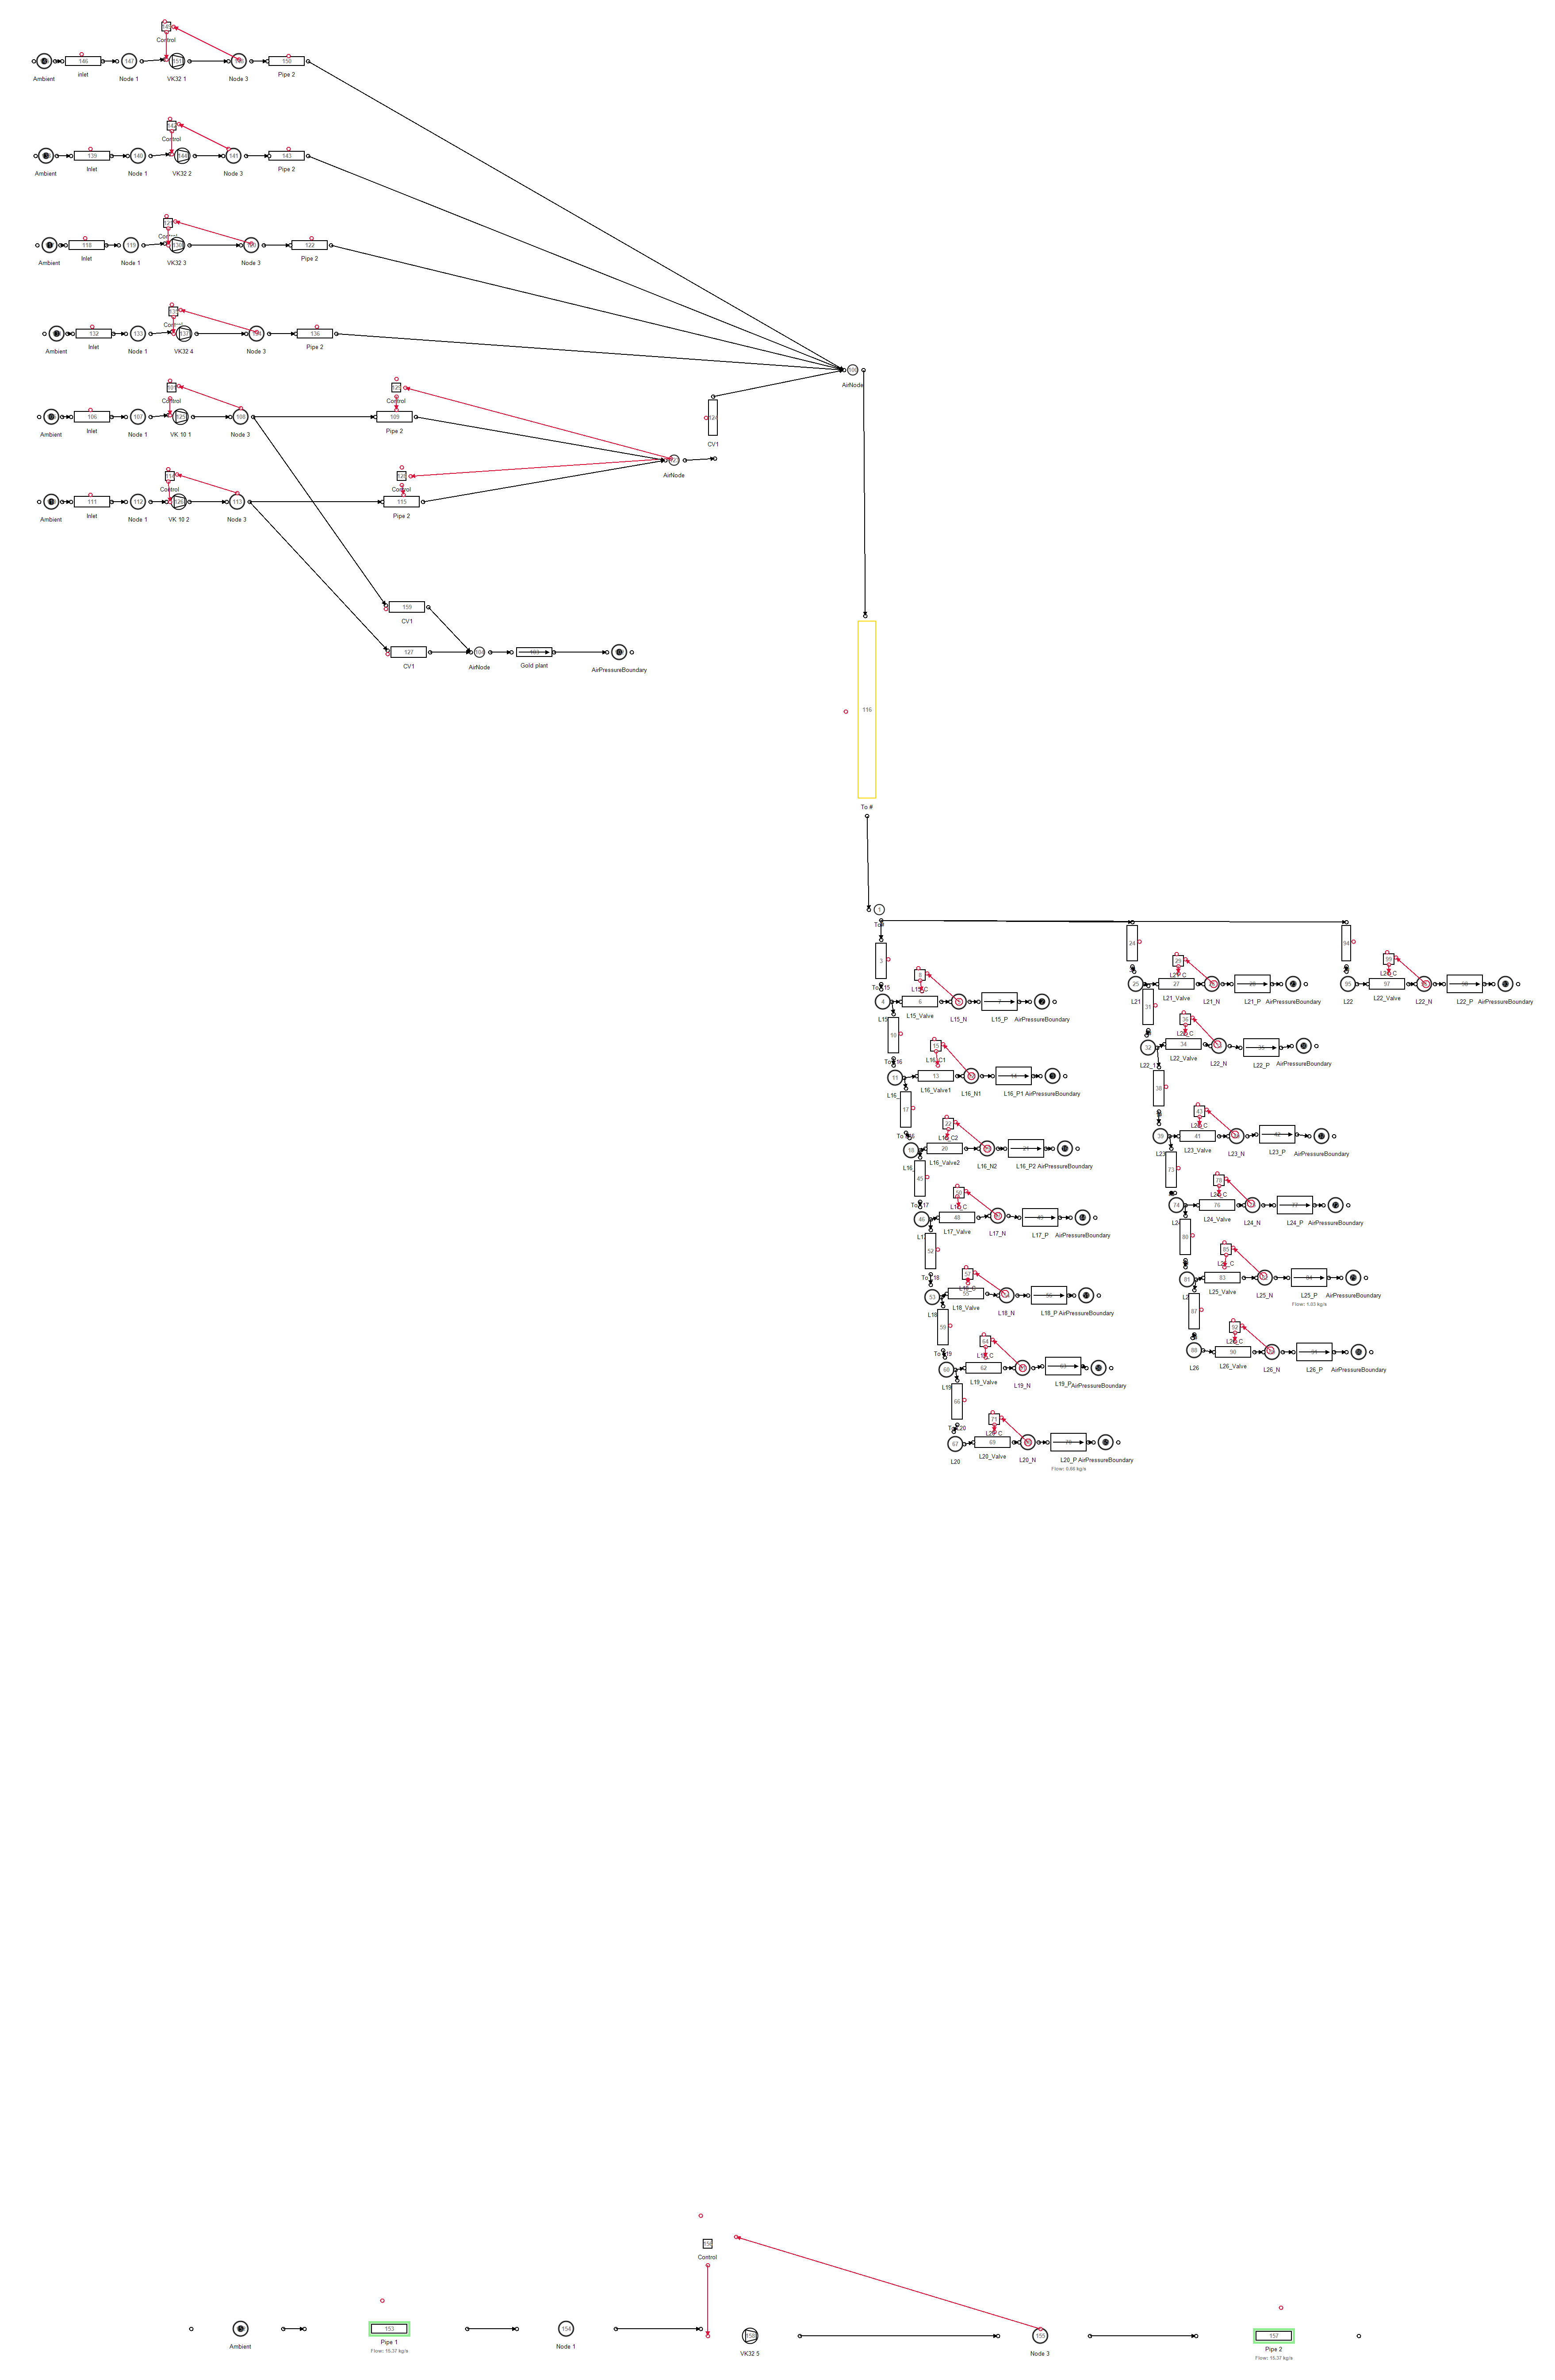
\includegraphics[width=\textwidth]{Images/A/BeetSim}}
		\caption{Mine A: Simulation model diagram}
		\label{fig: BEET Baseline model}
	\end{figure}

	\begin{figure}[h!]
		\centering
		\fbox{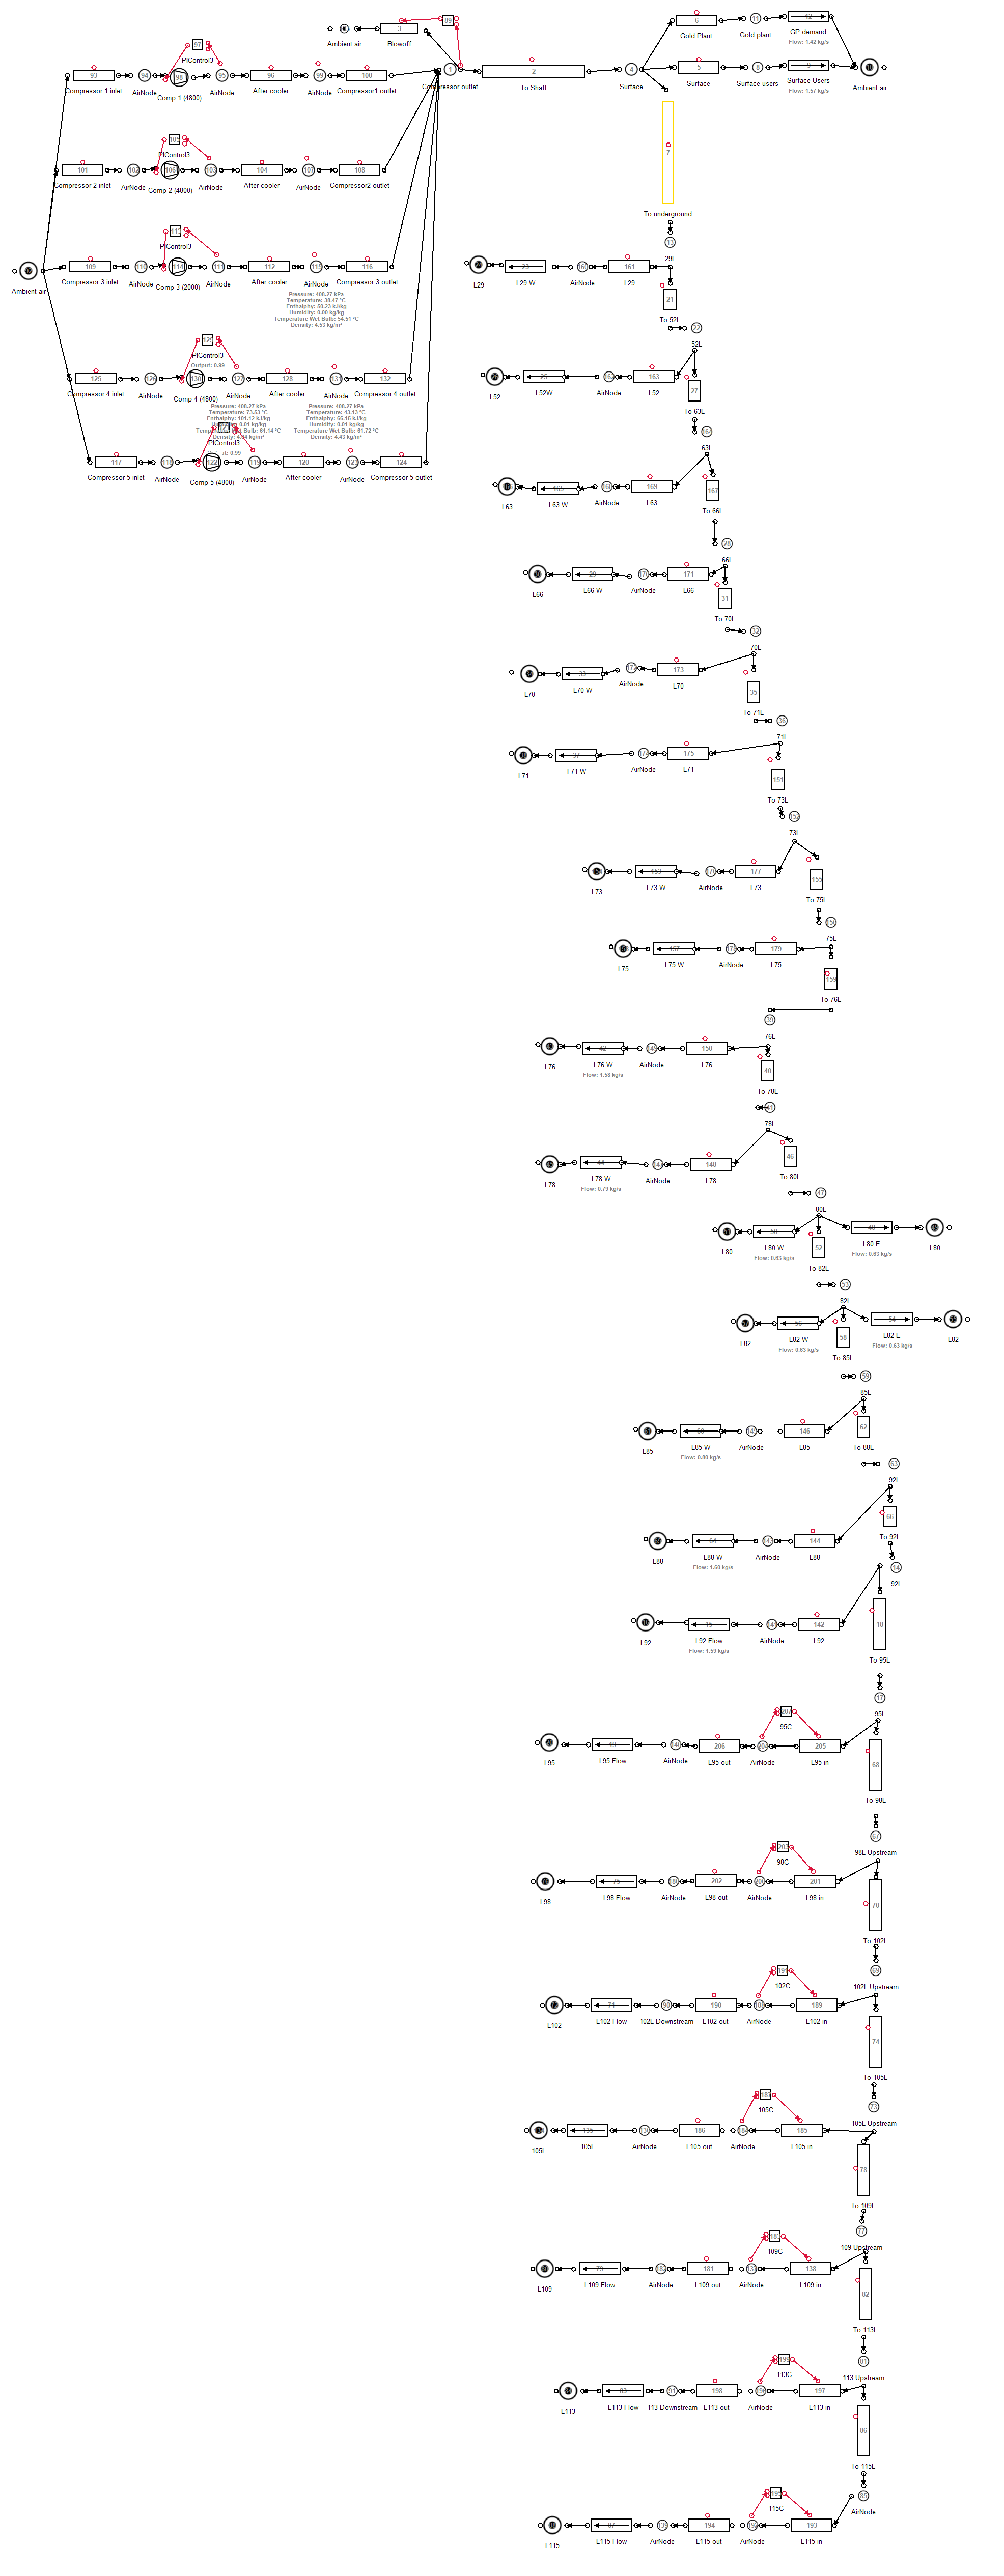
\includegraphics[trim =-20cm 0 -20cm 0cm,width=\textwidth]{Images/4/KUS_Basline2}}
		\caption{Mine B:  Baseline simulation model diagram.}
		\label{fig: KUS Baseline model}
	\end{figure}

	\begin{figure}[h]
		\centering
		\fbox{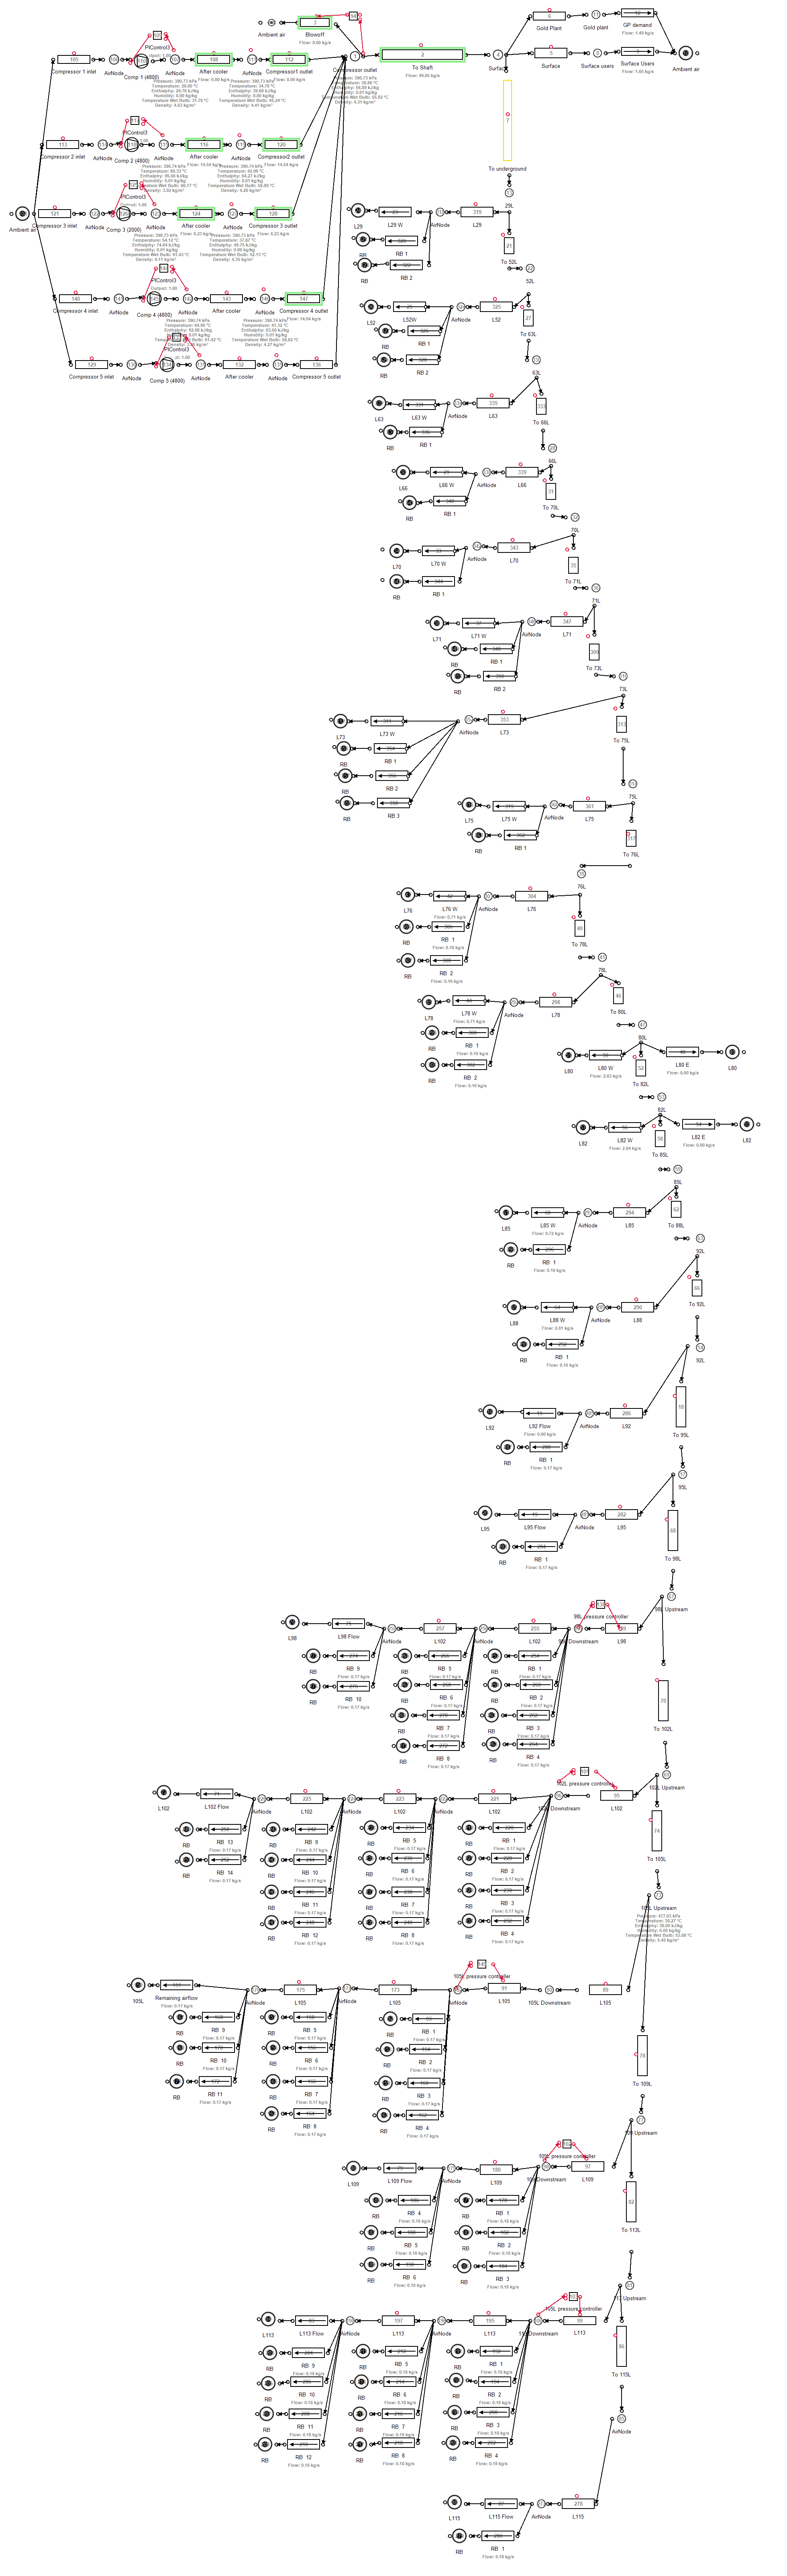
\includegraphics[trim =-35cm 0 -35cm 0cm,width=\textwidth]{Images/A/RefBaySim}}
		\caption{Mine B: Simulation model diagram for the refuge bay scenario.}
		\label{fig: Refuge bay layout}
	\end{figure}	

	\begin{figure}[h]
		\centering
		\fbox{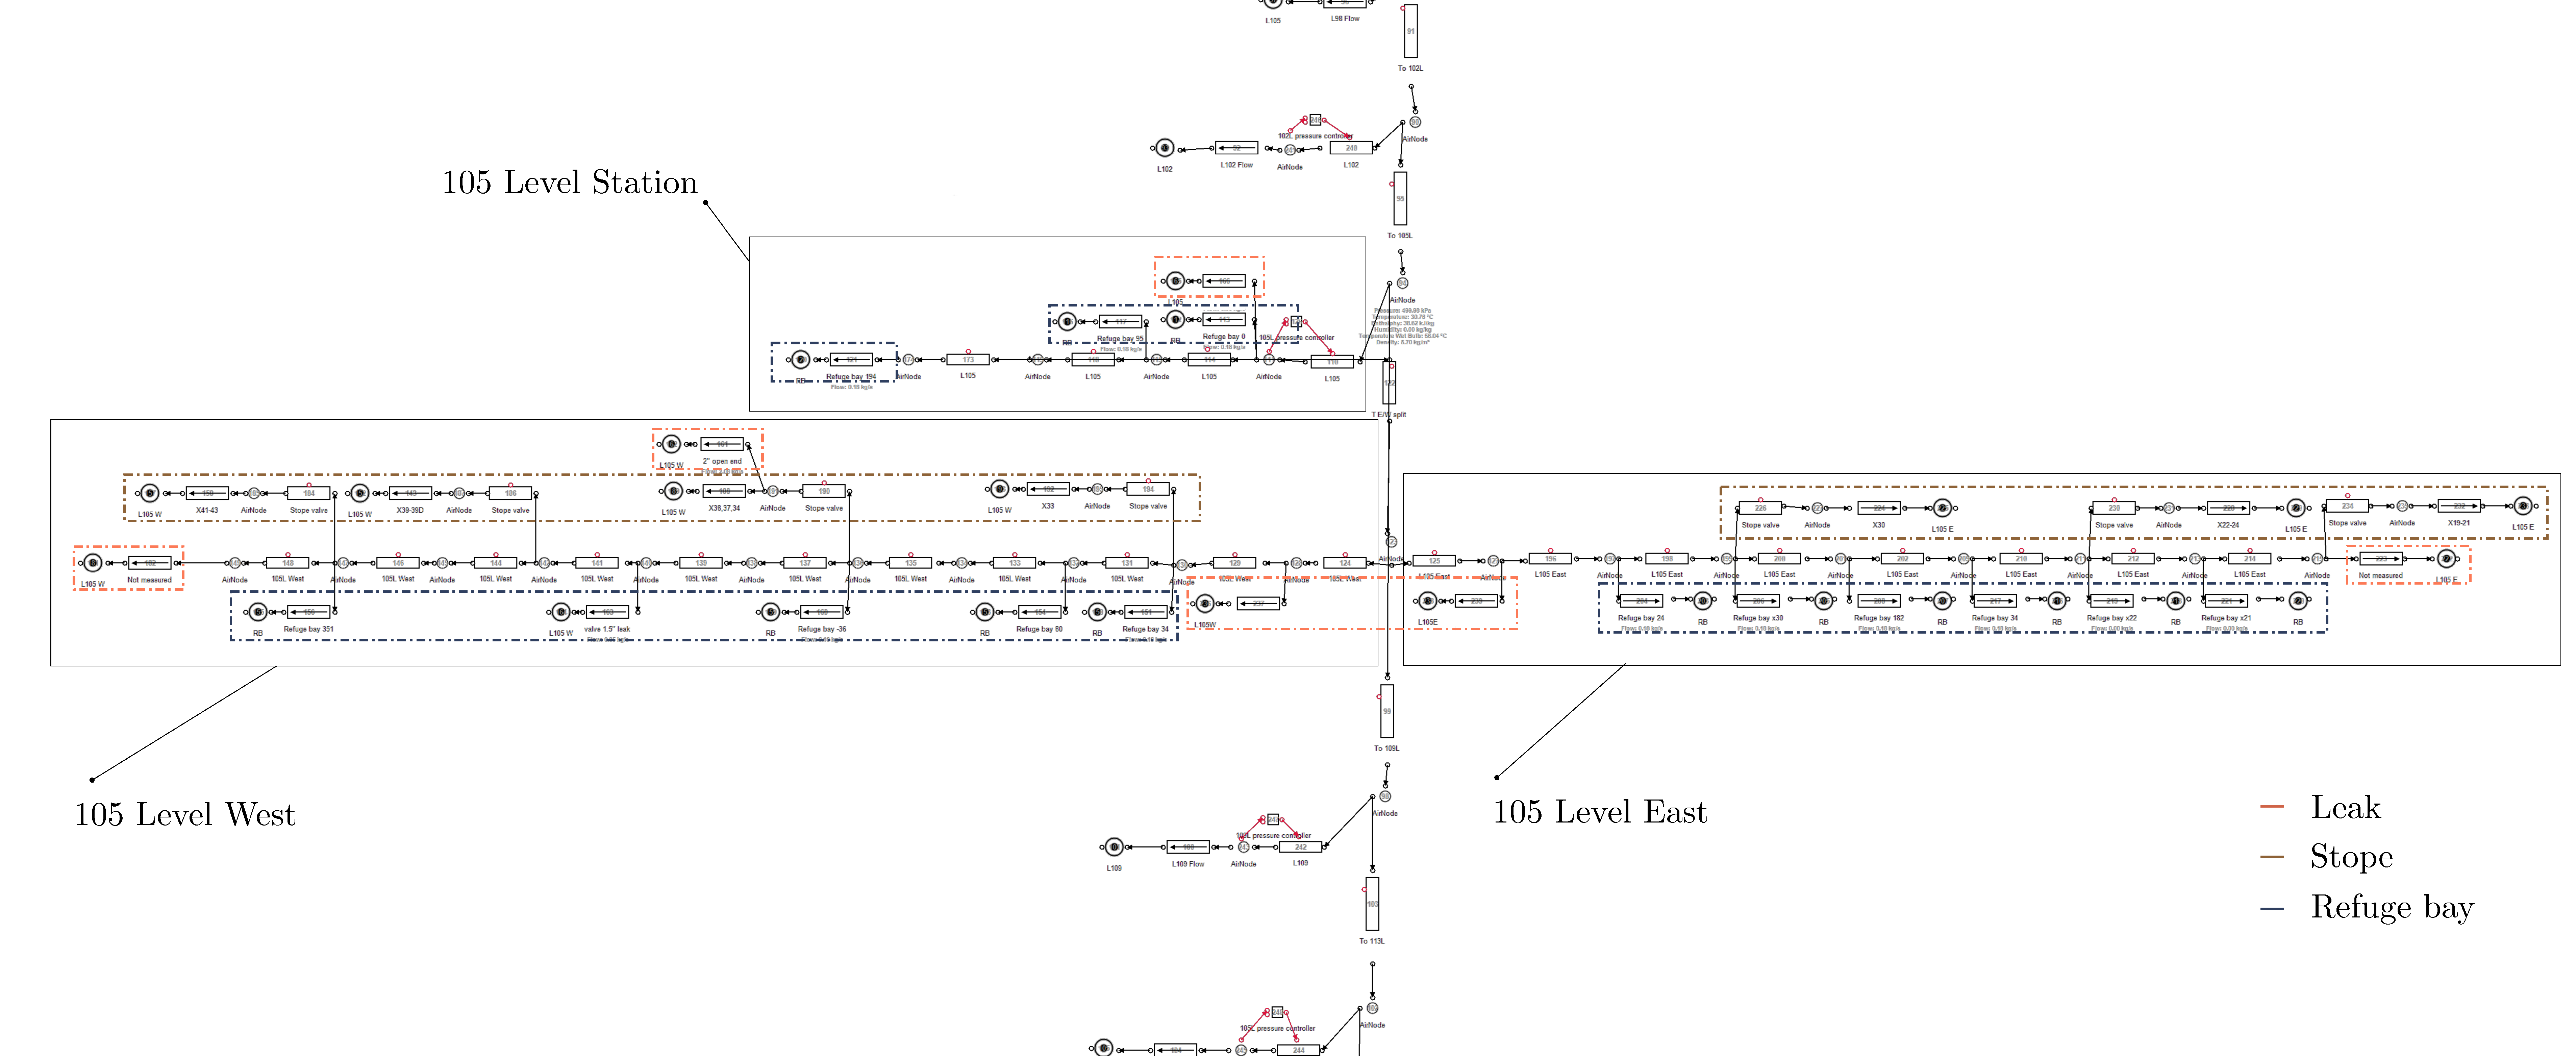
\includegraphics[,width=\textwidth]{Images/A/StopeSim}}
		\caption{Mine B: Simulation model diagram for the station isolation stope control.}
		\label{fig: Stope layout}
	\end{figure}

\end{appendices}
